\documentclass[conference]{IEEEtran}
%=====PACKAGES=====
\usepackage{amsmath,amssymb}		%To use math symbols
\usepackage{graphicx}				%To include figures
\usepackage[font=footnotesize]{caption}	%To specify the font of captions
\usepackage{soul}                   %for better underlines
\usepackage[table,xcdraw]{xcolor}


%=====SYMBOLS DEFINITIONS=====
\def \R{\mathbb{R}}
\def \X{\boldsymbol{\rm X}}
\def \y{\boldsymbol{\rm y}}
\def \bbeta{\boldsymbol{\beta}}
\def \T{\mathsf{T}}


%=====DOCUMENT=====
\begin{document}
\title{Automatic Segmentation of Pseudomonas Aeruginosa Biofilms Using a Deep Learning U-Net Framework}
\author{
\IEEEauthorblockN{Grant S. Roberts}
\IEEEauthorblockA{\sc{BMI/CS 567 Final Project}}
}
\maketitle

%=====ABSTRACT=====
\begin{abstract}
Accurate segmentation is critical for the quantification of structural and temporal characteristics of biofilm cultures and is of particular importance when monitoring a biofilm’s response to antibiotic treatment regimens. However, the large size of light microscopy images, as well as the large number of images that may be needed for proper cell-tracking over multiple biofilm strains, warrant automated means of segmentation to expedite post-processing and increase segmentation repeatability. In this study, a fully-convolutional neural network with U-Net architecture was trained to segment Pseudomonas Aeruginosa biofilm images using a total of 60 training and 10 validation datasets. This deep learning approach was compared to a “simple” manual segmentation using multi-vertex polygon ROI tracing. Both methods were compared to ground-truth biofilm images and quantitatively assessed using dice coefficients and modified Hausdorff distances to rate the efficacy of each method. Ground-truth images were obtained by producing an approximate mask using various morphological operations and by extensive manual fine-tuning of edges. Intra-observer repeatability of simple segmentation and ground-truth segmentation was assessed for 10 repeat datasets using intraclass correlation coefficients. It was found that ground-truth manual segmentation was extremely time-consuming, taking on average 23 minutes while simple segmentation took on average 1 minute. Deep learning segmentation resulted in fairly low accuracy, as measured by dice coefficients and Hausdorff distances. Further studies utilizing different frameworks, better computational resources, and augmented datasets are highly warranted in order to provide increased accuracy of automatic deep learning segmentation of biofilm images.
\end{abstract}



%=====INTRODUCTION=====
\section{Introduction}
\label{secName}
Biofilms are large aggregations of microorganisms encased in a matrix of extracellular polymeric substance that grows on the surface of certain materials [1]. This complex grouped structuring, described by some as a "city for microbes", allow for efficient biochemical signaling and gene exchange and provides protection against external stresses, increasing overall cell survival rates [2]. Biofilms are extremely robust to external stresses, capable of growing on many different surfaces and showing resistance towards some forms of antibiotics and detergents, which is particularly problematic in the medical context [3, 4]. These biofilm colonies can readily grow on surgical equipment and soft tissue wound infections, with some data suggesting that they may account for approximately two-thirds of chronic microbial infections [5, 6]. Treatment or removal of biofilms, whether in-vivo or ex-vivo, is exceptionally difficult and often involves a regimen of multiple forms of high-strength antibiotics due to a lack of knowledge of the exact bacterial strain present and the degree of antibiotic resistance. While conventional antibiotic resistance (associated with evolutionary adaptation towards antimicrobials) may play a role in limiting the treatment efficacy of antibiotics, evidence is beginning to suggest that it may be more related to inherent, multi-layered stress responses (formation of persister cells, nutrient limitation, slow growth, etc.) within the biofilm [7]. However, these adaptive defense mechanisms are still poorly understood. In order to develop more targeted treatment strategies, it is thus imperative to prospectively characterize the morphological and functional responses that occur during antibiotic challenges. 

To better understand structural and temporal changes of biofilms in response to antibiotic challenges, microscopy techniques (namely optical microscopy and confocal laser scanning microscopy) have been used to obtain high-resolution digital images of live bacteria strains grown on hard agar plates [8, 9]. This high-resolution imaging can allow for accurate tracking of morphological changes over time and can allow for visual differentiation in gene content and expression amongst various biofilm strains. In order to perform data analysis, accurate image segmentation of the biofilm is required. This segmentation is commonly performed using several software platforms, which rely on either manual thresholding [10, 11] or automatic thresholding [12-14] to differentiate between regions of biofilm and agar background. Both approaches are prone to error, as manual thresholding may produce subjective results and show poor repeatability and automatic thresholding may be negatively influenced by erroneous pixels, artifacts, and differences in background lighting [14, 15]. Deep learning has emerged as a compelling approach to segment biomedical images, as well as biofilms, using trained convolution neural networks [16, 17].

In this paper, a fully-convolution neural network with U-Net architecture will be used to automatically segment Pseudomonas Aeruginosa biofilm images. The accuracy of this technique will be compared to a “simple” manual segmentation technique, in which multi-vertex polygons are drawn around the biofilm to quickly create a crude ROI. While the simple segmentation will include the entirety of the biofilm, the edge structures, which may contribute a significant amount of area, will not be accounted for. Thus, it is hypothesized that the U-Net segmentation scheme will provide a robust means to accurately segment biofilms and preserve complex edge structures. If successful, this method would allow for fast and formidable segmentations with increased repeatability, reproducibility, and accuracy of biofilm measurements, necessary for the characterization of the complex functional and structural changes of biofilms that may occur under the stress of antibiotic treatments.

%=====DATA=====
\section{Data}
A total of 266 two-dimensional (2D) color (3-channel RGB) digital JPEG images were downloaded from a shared online folder. This dataset contained 69 different strains, each strain containing 3-4 images obtained at different time points after the administration of antibiotics. Due to the time-consuming nature of manual segmentation required for ground-truth measurements, only 70 of these images were used for analysis. This sub-dataset contained 18 different strains; 16 strains contained 4 time-series images while 2 strains contained 3 time-series images (total 70 images). Color images in the sub-dataset varied in file size (mean: 28.3 MB; range: [8.27-62.9] MB) and dimension (mean: 7155x7721x3 pixels; range: [4440-13080]x[5376-14016]x3 pixels). A representative biofilm image from the sub-dataset is shown in Figure \ref{figName1}. MATLAB 2020a (Mathworks, Natick, MA, USA) was used to import and manipulate raw images. All images were converted to a standardized size of 8192x8192 prior to manual, simple, and U-net segmentation. 

\begin{figure}[h]
\centering
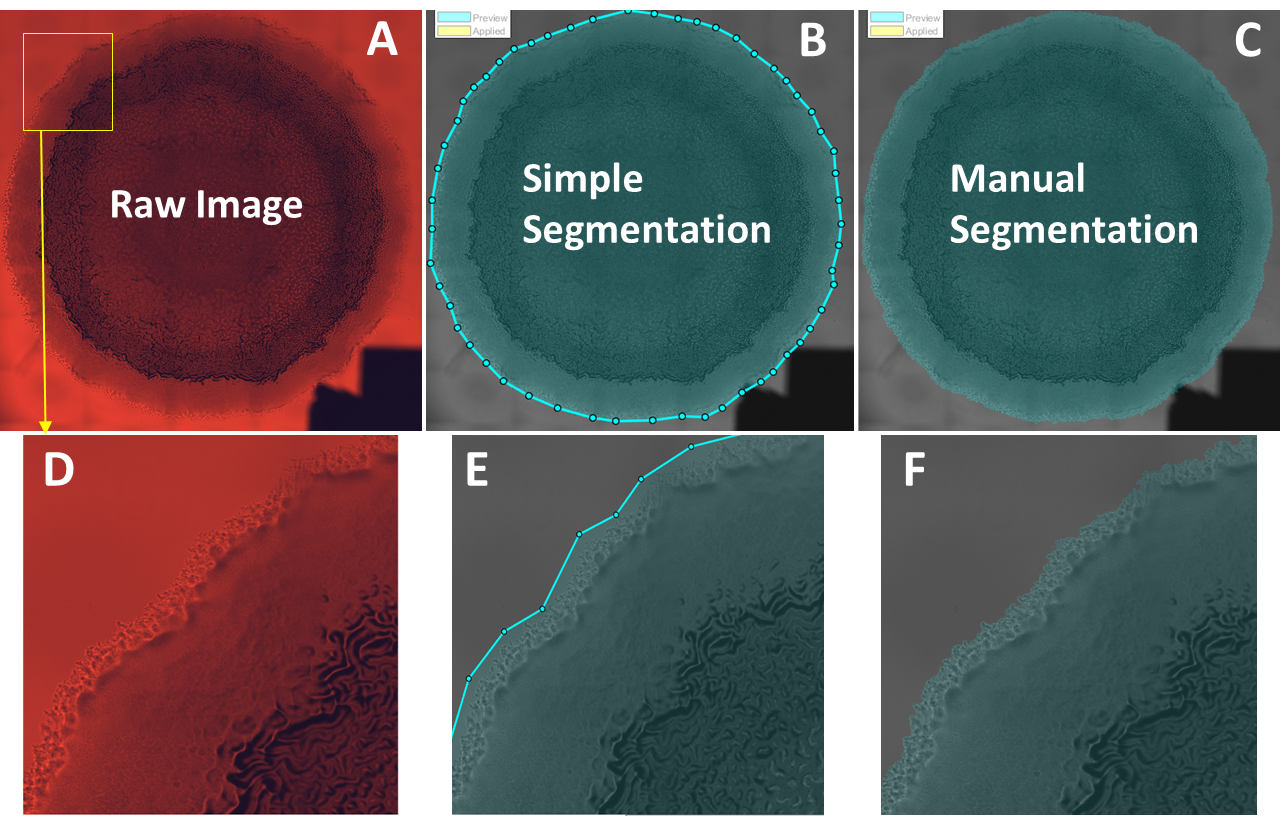
\includegraphics[scale=0.25]{Slide1.PNG}
\caption{Figure 1: (A) Stained microscopy image of biofilm culture on agar plate. (B) Multi-vertex polygon ROI traced around biofilm boundary. (C) Manual segmentation of biofilm using free-hand region of interest (ROI) tracing. (D-F) Zoomed images of biofilm boundaries, with associated segmentation ROIs.}
\label{figName1}
\end{figure}


Simple segmentation masks were performed on all 70 datasets. Masks were subsequently saved as 8192x8192 binary 8-bit TIF files. TIF files were used because it was noted that JPEG files resulted in lossy compression; while the image appeared binary, closer inspection revealed that pixels were non-binary grayscale.  Manual segmentation ground-truth masks were created for all 70 datasets and were subsequently saved as 8192 x 8192 binary 8-bit TIF files. For U-Net segmentation, 60 images (85\%) were assigned as training datasets and the remaining 10 images (15\%) were delegated for validation. 

%=====METHODS=====
\section{Methods}
\ul{Manual Segmentation}: Manual segmentation masks were created for ground-truth images, used for quantitative segmentation performance evaluation and U-Net training. Initially, the raw color images were converted to grayscale, as was done for simple segmentation. A second gradient magnitude image was then obtained by convolving the grayscale image with a 3x3 Sobel gradient kernel and taking the magnitude of all pixels. A third image was created by taking the log of gradient magnitude image and performing a subsequent Wiener smoothing filter to mitigate noise in the background regions caused by the log operation. All three images were then resized from the initial image dimensions to the standardized size of 8192x8192. Two separate methods were used to create an initial mask depending on the image characteristics of the gradient and log-gradient image. If the gradient image showed good delineation of the biofilm boundary, then a manual threshold was used to include only the edge and center of the biofilm, as these regions showed more image variation (as opposed to the slowly varying background region). This method was used on 45 (of the 70 total datasets). If the log-gradient showed a better delineation of the biofilm boundary, a flood-fill operation was performed on the interior of the biofilm. This method was used in 25 of the datasets. After creation of the initial mask, holes inside of the biofilm and small regions of active pixels outside of the biofilm still existed. To create a uniform mask, holes (areas of nonactive pixels surrounded completely by active pixels) were filled using a built-in hole-filling algorithm. Next, a small line of active pixels was created, leading from the edge of the image to the center of the biofilm, and the mask was inverted. The line was drawn because, after inverting the mask, the central region (biofilm) would often become filled after performing the hole-filling operation due to (now active) background pixels surrounding the central region. The artificial line created a non-active pixel channel, forcing the central region to not be completely enclosed while still filling in noise holes in the background region. The artificial line was then removed through manual segmentation. Finally, the mask was inverted again, leaving a mostly uniform mask with no holes or noisy background spots. This procedure is visually shown in Figure \ref{figName2}. A morphological opening operation, utilizing a disk of radius 3 pixels, was performed to connect disjointed regions near the edge of the biofilm. Despite this, crevices within the edge structure were often filled and certain regions of low edge contrast were poorly segmented. Because of this, manual fine-tuning of the edge was performed using a free-hand ROI tracing. This procedure was performed on all 70 images in the sub-dataset by an imaging scientist with 3+ years of experience in image segmentation and image processing. A manually segmented image is shown in Figure \ref{figName1}.

\begin{figure}[h]
\centering
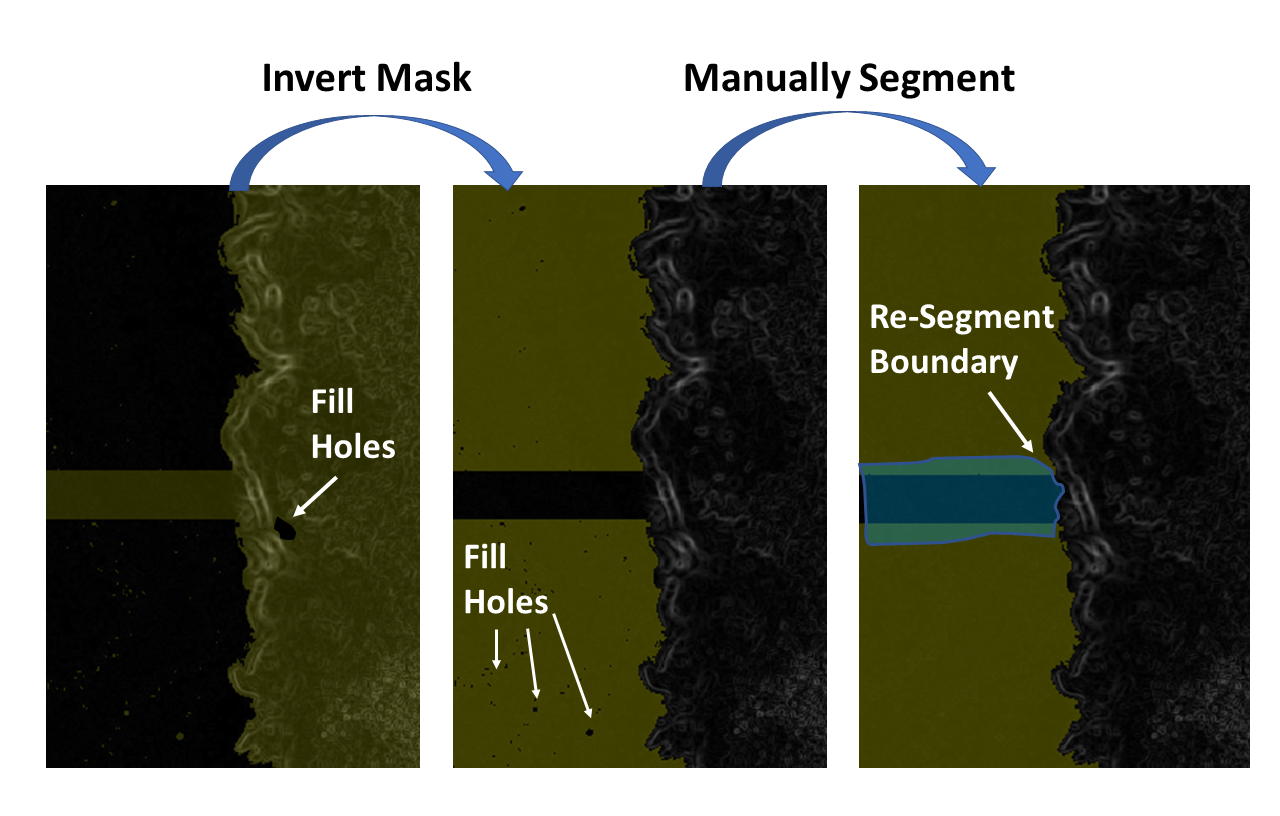
\includegraphics[scale=0.25]{Slide2.PNG}
\caption{Figure 2: Pre-processing procedure performed before manual segmentation to create uniform ROI without holes or noise spots. Hole-filling is first performed on the manually-thresholded or flood-filled biofilm area. Immediately after this, an artificial line is drawn from the biofilm ROI to the image edge. Next, the image is inverted and the hole-filling operating is performed again, removing noise pockets in the background region. The artificial line that was drawn creates a disconnect within the background region, which allows hole-filling to not fill the main biofilm area. Lastly, this artificial line is removed by manual segmentation.}
\label{figName2}
\end{figure}

\ul{Segmentation}: A simple segmentation procedure, utilizing a multi-vertex polygon region of interest (ROI) tracing, was performed in the Image Segmentation Toolbox in MATLAB 2020a. This segmentation was intended to be quick and crude, with little attention given to the high-detail boundaries. Before simple segmentation was performed, all images were converted to grayscale by weighting the red component by 0.2989, the green component by 0.5870, and the blue component by 0.1140 and summing the respective channels. The black-white image was then loaded from the workspace into the toolbox, and an ROI was contoured around the biofilm. The number of vertices used, as well as the time required to produce the ROI, was recorded. This procedure was performed on all 70 images in the sub-dataset by the same user. A representative multi-vertex polygon ROI is shown in Figure \ref{figName1}. 

\begin{figure}[h]
\centering
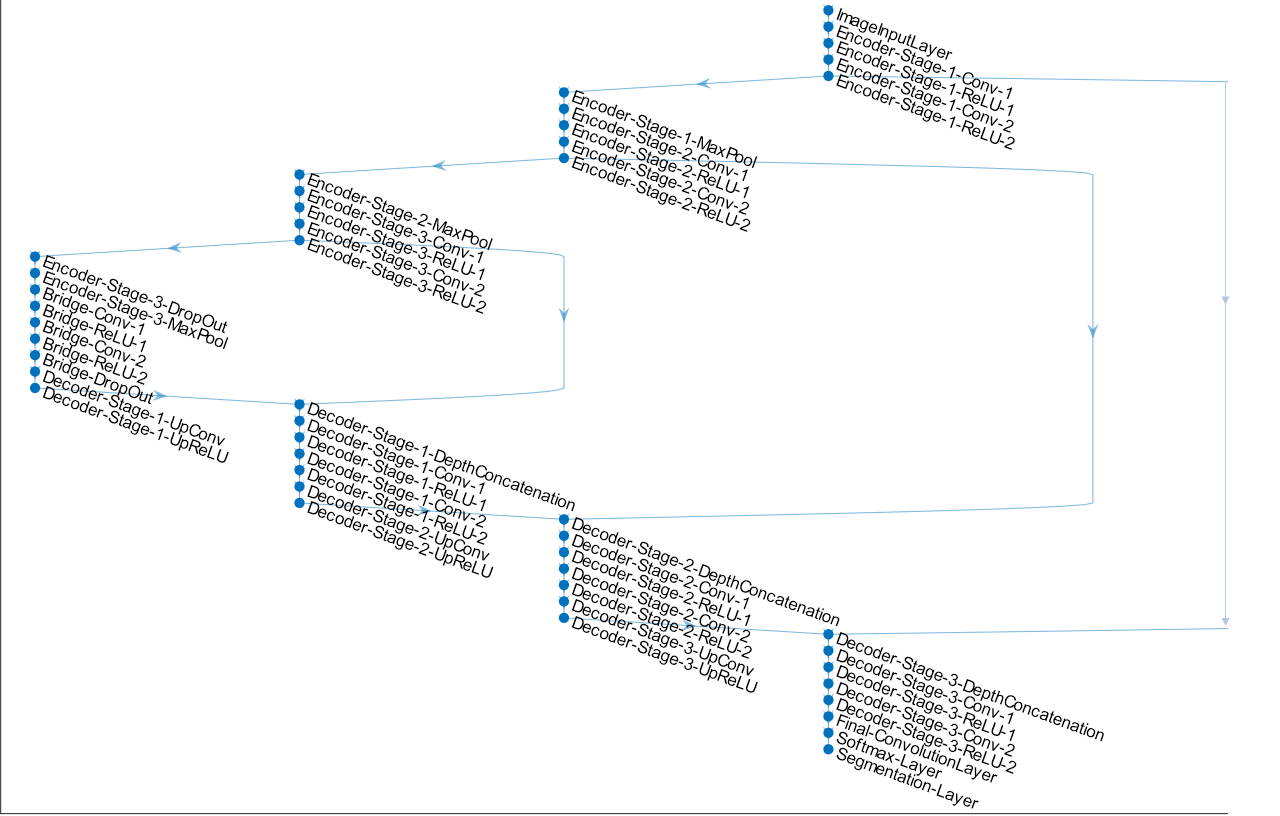
\includegraphics[scale=0.25]{Slide3.PNG}
\caption{Figure 3: A MATLAB plot of the U-Net architecture diagram used in this study.}
\label{figName3}
\end{figure}

\ul{U-Net Segmentation}: A U-Net architecture was constructed in MATLAB 2020a using the Computer Vision and Deep Learning Toolboxes. Specifically, the function ‘unetLayers’ was used to construct this architecture, shown in Figure \ref{figName3}. It was fully convolution, utilizing an encoding depth of 3, mini-batch size of 8, with color image input and binary (two-class) output. Due to the large image sizes, image patches of size 256x256 were randomly extracted from the training and validation images and were fed into the network input. A cross-entropy loss pixel classification layer was used as the final layer in the network. A piecewise learning rate schedule was used, with an initial learning rate of 5e-04, learning rate drop period and drop factor of 5 and 0.95, respectively. Training progress was plotted in a graphical user interface, shown in Figure \ref{figName4}.  The network was trained over 20 epochs with validation occurring every 400 iterations. Due to limited computing resources, training was performed remotely on a Dell Precision 5820 Tower (Intel Xeon W-2123 3.60 GHz CPU, 32 GB RAM, NVIDIA GeForce GTX 750 Ti GPU [Nvidia Corporation, Santa Clara, CA, USA] with 2 GB memory and 1020 MHz core speed). Lastly, segmentation prediction outputs from the network were post-processed to remove checkerboard pattern artifacts visible on some images, as well as disjointed boundary regions, leading to the final segmentation image. This procedure was performed on all 70 images in the sub-dataset and the subsequent masks were saved as TIF files. 

\begin{figure}[h]
\centering
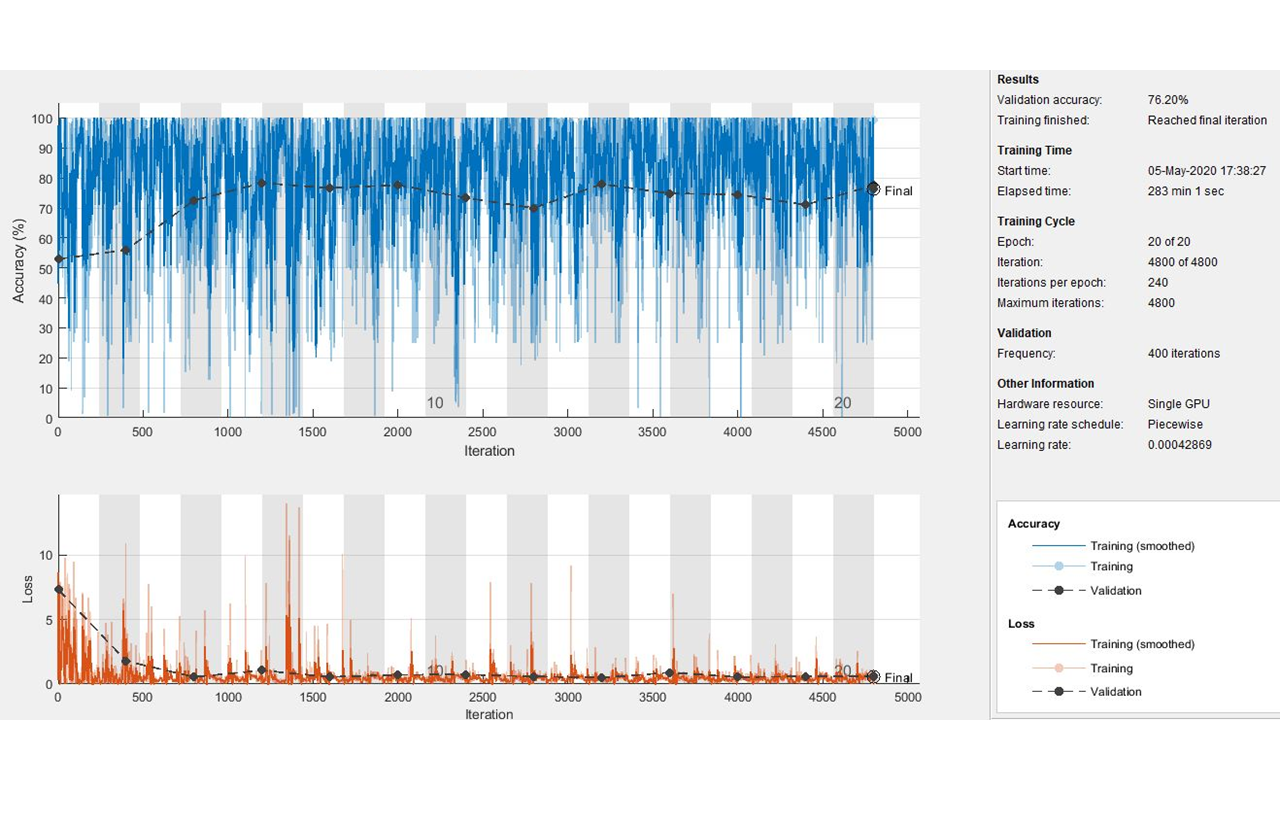
\includegraphics[scale=0.25]{Slide4.PNG}
\caption{Figure 4: A built-in MATLAB graphical user interface (GUI) of the training progression. The top graph depicts the accuracy of the training data relative to ground-truth segmentations, and the bottom graph depicts the loss function over each iteration. The sidebar on the right shows what stage of the training you are in, computational resources that are utilized, as well as the total time-elapsed.}
\label{figName4}
\end{figure}

\ul{Image Analysis}: Dice coefficients were used to compare segmentation accuracy between the simple and U-net segmentation methods, relative to the ground-truth manual segmentations. An additional accuracy metric, the modified Hausdorff distance (MHD), was calculated for both the simple and U-Net segmentations relative to ground-truth. Due to the use of max and min functions in the original Hausdorff distance measure, the presence of a single noisy outlier can drastically change the Hausdorff measurement, limiting its practical applications. The ‘modified Hausdorff distance’ overcomes this problem and was shown to perform well even in noisy datasets [18]. Average area measurements (reported as a percentage of total area) were calculated for all simple, U-Net, and manual segmentations. 

\ul{Repeatability Analysis}: Ten repeat manual and simple segmentations were performed by the same user 2 days after the initial segmentation to assess intraobserver repeatability. Intraclass correlation coefficients were used as a metric to asses repeatability for both the manual and simple segmentation methods, using a significance level of 0.05. Furthermore, Dice coefficients between the two measurements were calculated between the initial and repeat segmentations. 


%=====EXPERIMENTS=====
\section{Experiments}
Seventy images were successfully segmented for all techniques and were saved as binary masks. Additionally, a deep learning model was successfully trained on these datasets with segmentation prediction masks obtained. Figures 5-7 show a simple, U-Net, and manual segmentation of several biofilm images. Quantitative segmentation performance results for the simple and U-Net segmentation methods are reported in Table 1. The times required for segmentation are also reported in this table.

\begin{figure}[h]
\centering
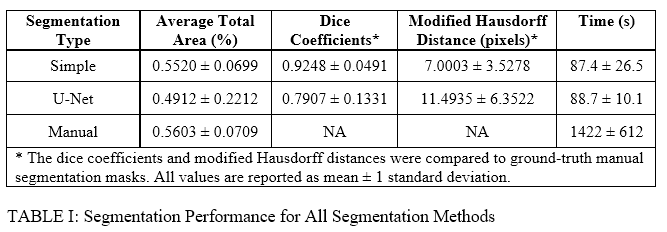
\includegraphics[scale=0.5]{Table1.PNG}
\label{Table1}
\end{figure}

\begin{figure}[h]
\centering
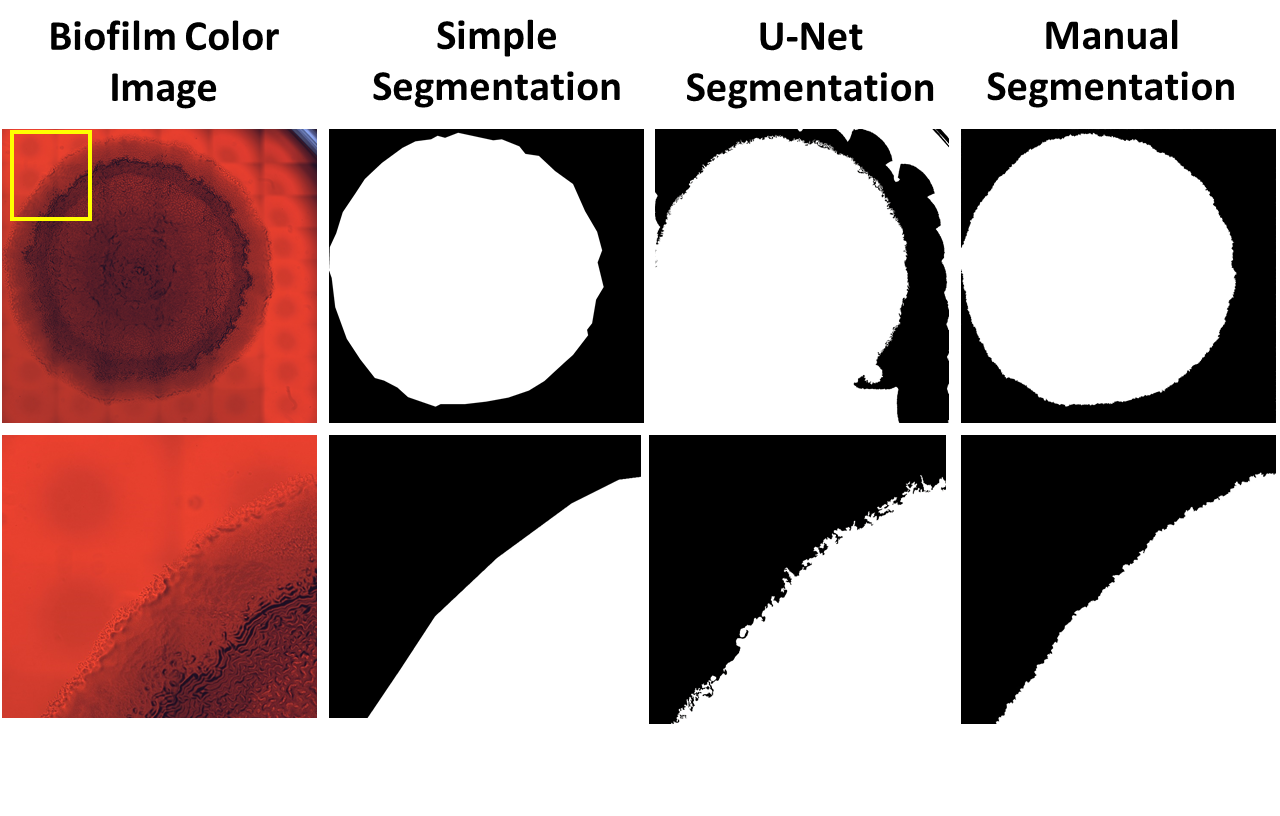
\includegraphics[scale=0.25]{Slide5.PNG}
\caption{Figure 5: Biofilm (Strain 1) showing simple, U-Net, and manual segmentations. The bottom images show a close up of the biofilm boundary.}
\label{figName5}
\end{figure}

\begin{figure}[h]
\centering
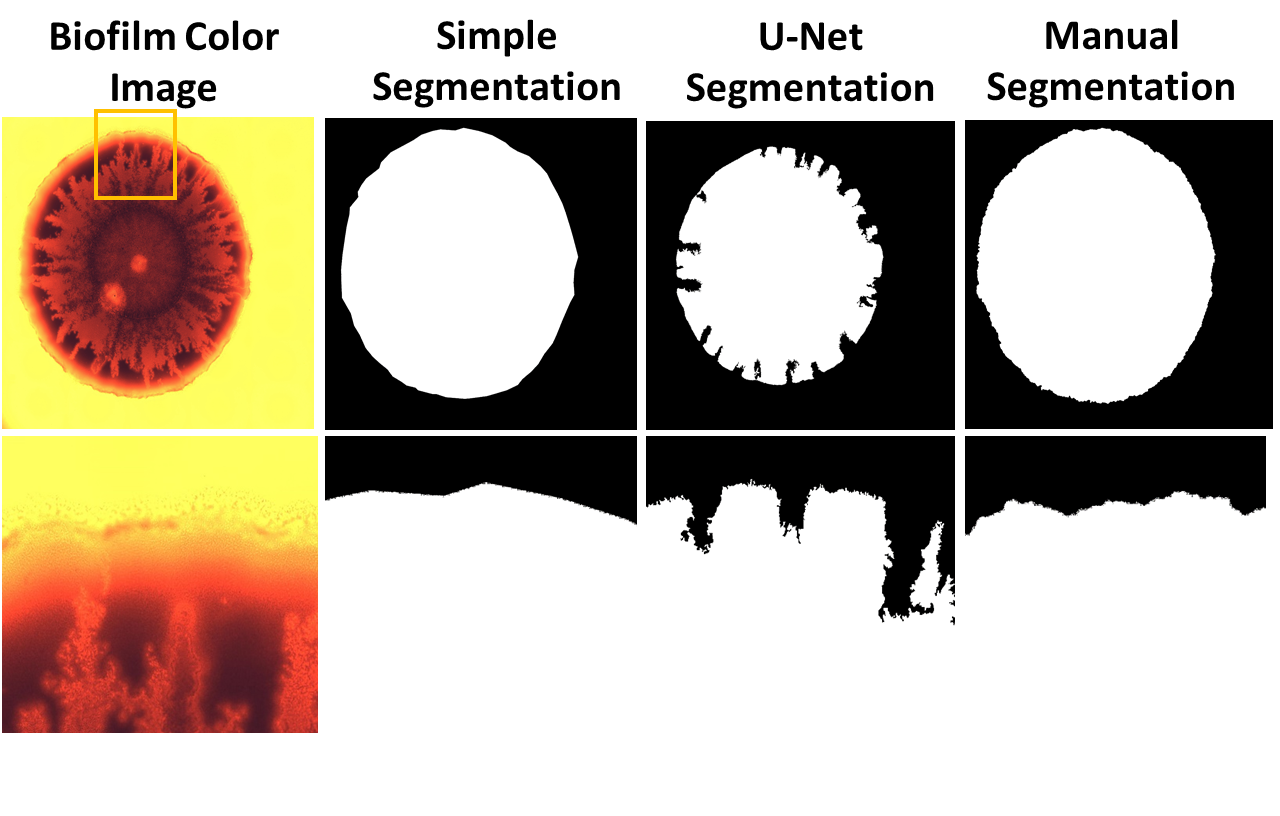
\includegraphics[scale=0.25]{Slide6.PNG}
\caption{Figure 6: Biofilm (Strain 25) showing simple, U-Net, and manual segmentations.}
\label{figName6}
\end{figure}

\begin{figure}[h]
\centering
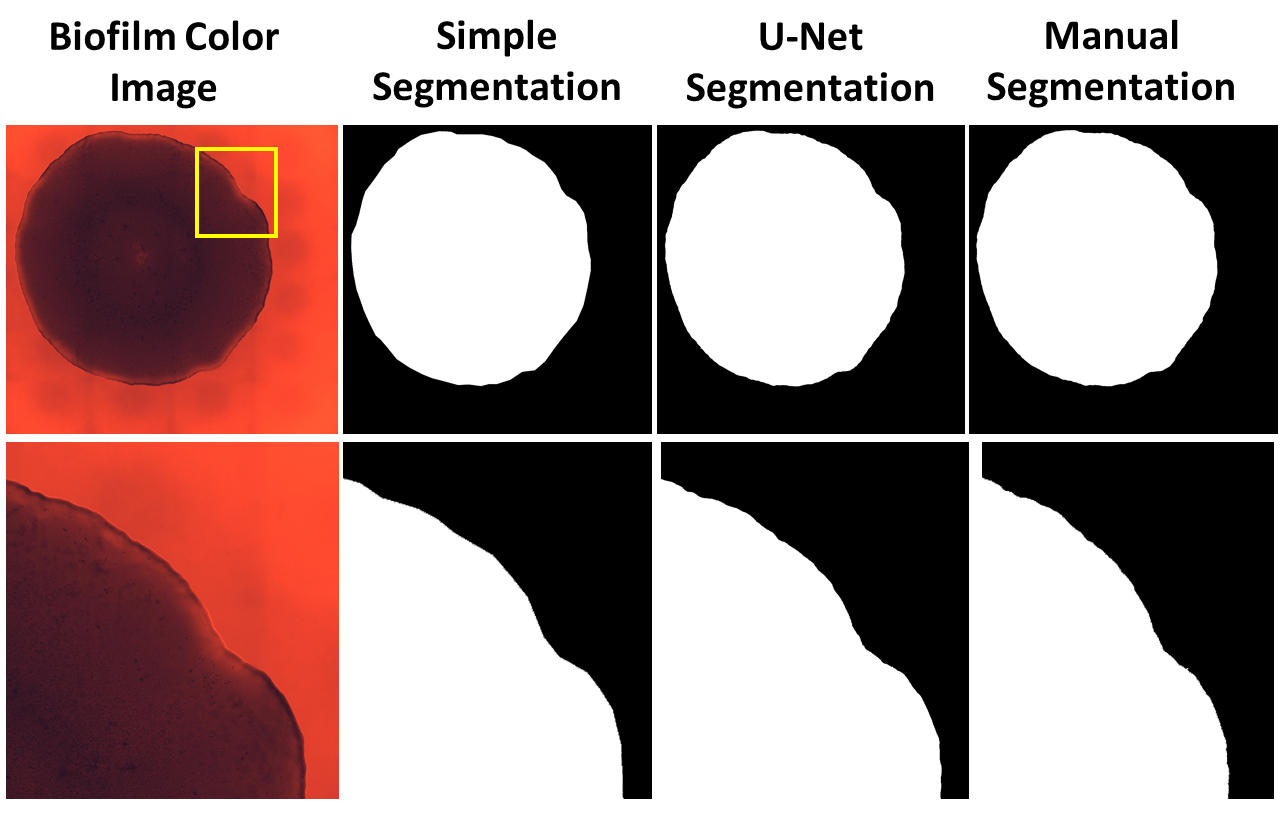
\includegraphics[scale=0.25]{Slide7.PNG}
\caption{Figure 7: Biofilm (Strain 41) showing simple, U-Net, and manual segmentations.}
\label{figName7}
\end{figure}

\ul{Manual Segmentation}: While the initial mask created using morphological operations did a good job at creating an accurate segmentation, certain regions on the edge of the biofilm were often disjointed and noisy. While morphological opening addressed these issues, it also removed the true edge in areas of low image contrast. Performing manual trimming helped create accurate tracing around the edges. However, this process was extremely time-consuming, requiring on average 23.7 $\pm$ 10.2 minutes per dataset. Intraobserver repeatability of the 10 repeat manual segmentations was particularly high, with an average dice coefficient of 0.9984 $\pm$ 0.0019 and an intraclass correlation coefficient of 0.9995.

\ul{Simple Segmentation}: Segmentation difficulty increased moderately when images with non-smooth edges were presented, increasing both the number of vertices and time required to process the image. Images were segmented at full scale, leading to difficult visualization of the true biofilm boundary in some datasets. However, the average time to trace the polygon ROI was still quite fast, requiring on average 73.2 $\pm$ 21.2 seconds and an average of 87.4 $\pm$ 26.5 vertices. While it was initially hypothesized that the simple segmentation would result in poor segmentation accuracy, the simple segmentation actually outperformed the deep learning segmentation on all metrics. Furthermore, intraclass correlation coefficients were 0.9975 for the 10 repeated simple segmentations, indicating very high intraobserver repeatability for this method. Dice coefficients between the initial and repeat segmentation masks also indicated very high repeatability with an average coefficient of 0.9929 $\pm$
 0.0026. While the segmentation accuracy and repeatability were high (relative to the U-Net segmentations), the true edge boundaries were not well preserved.

\ul{U-Net Segmentation}: The total time to train the network took approximately 5 hours to complete. This made testing of different parameters and layers extremely difficult, which is likely a reason why the performance of the deep learning segmentation was lower than the simple segmentation. Upon initial training, the ground-truth masks were saved as JPEG files. However, as noted above, saving the masks as JPEG files resulted in lossy compression, causing the binary masks to be non-binary in certain areas, causing the training accuracy to be greatly decreased. Manual segmentations were then saved as TIF files, which maintained the binary nature of the ground-truth masks and resulted in much higher training accuracy. Segmentation accuracy, as measured by Dice coefficients and modified Hausdorff distances were quite low. Qualitatively, many of the segmentation masks produced could not detect low contrast edges. Therefore, in many of the U-Net produced masks, there exist large fragmented edge regions. It was also noted that in some instances (N=6), the segmentation prediction resulted in a mask that covered the entire image. In these images, the luminance was quite low, and the background region contained large artifacts. Despite this, the time to perform segmentation after network training was relatively fast, taking approximately 90 seconds.

\ul{Limitations}: While the manual segmentations were performed by a user with experience in image segmentation and image processing, further validation of the ground-truth images should be performed by a microbiologist specializing in this field. For instance, in some image datasets, a very low contrast, rough edge was observed to exist outside of a higher contrast smooth edge. It is unclear whether this outer rough edge is truly the biofilm boundary or an extension of the extracellular polymeric substance matrix. Due to a lack of access to high computing power machines, training of the network was slow and required a great deal of modifications to reduce the memory load. Using multiple GPUs with greater processing capabilities would likely expedite the training process, allowing for more parameters to be changed and leading to overall improved accuracy. Additionally, this would result in increased memory, which could allow for loading in patches of larger sizes which may further improve the accuracy. Due to time limitations, data augmentation was not used. However, this approach would provide more datasets for training and would likely improve results. It is also theorized that adding further dimensionality to the color images, such as adding the gradient magnitude or log-gradient magnitude images in the fourth dimension may also lead to better segmentation predictions, as these images highlight biofilm boundaries quite well. Lastly, all images were resized to 8192x8192 to standardize resolution which led to decreased resolution through downsampling in some image datasets. 


%=====CONCLUSIONS=====
\section{Conclusions}
The accurate segmentation of biofilms is a difficult process; however, it is necessary in order to quantitatively characterize the complex functional and structural changes that occur under the stress of antibiotic treatments. While a previous study demonstrated high accuracy of biofilm image segmentation using a U-Net architecture, the U-Net segmentation in this study performed quite poorly. In fact, the simple segmentation method, in which polygons were manually traced around the biofilm, showed higher accuracy. The decreased performance is likely due to several factors, including lack of proper computation resources needed for fast training, as well as a low number of training datasets. Fortunately, these factors can be addressed through the use of high-power GPUs and data augmentation techniques, allowing for more datasets to be tested without having to perform tedious manual segmentation. To conclude, while this study demonstrated showed poor performance of the U-Net segmentation, much more extensive testing, training, and a carefully crafted neural net architecture would likely greatly increase the accuracy of this segmentation method, which would provide a highly repeatable means to segment biofilm cultures. 

%=====REFERENCES=====
\begin{thebibliography}{1}

\bibitem{paperName}
R. M. Donlan, \emph{Biofilms: microbial life on surfaces}, Emerging infectious diseases, vol. 8, no. 9, pp. 881-890, 2002.

\bibitem{paperName}
D. L\'opez, H. Vlamakis, and R. Kolter, \emph{Biofilms}, Cold Spring Harbor perspectives in biology, vol. 2, no. 7, pp. a000398-a000398, 2010.

\bibitem{paperName}
P. S. Stewart, and J. William Costerton, \emph{Antibiotic resistance of bacteria in biofilms}, The Lancet, vol. 358, no. 9276, pp. 135-138, 2001.

\bibitem{paperName}
P. N. Markham, and A. A. Neyfakh, \emph{Efflux-mediated drug resistance in Gram-positive bacteria}, Curr Opin Microbiol, vol. 4, no. 5, pp. 509-14, Oct, 2001.

\bibitem{paperName}
K. Lewis, \emph{Riddle of biofilm resistance}, Antimicrob Agents Chemother, vol. 45, no. 4, pp. 999-1007, Apr, 2001.

\bibitem{paperName}
M. Jamal, W. Ahmad, S. Andleeb, F. Jalil, M. Imran, M. A. Nawaz, T. Hussain, M. Ali, M. Rafiq, and M. A. Kamil, \emph{Bacterial biofilm and associated infections}, J Chin Med Assoc, vol. 81, no. 1, pp. 7-11, Jan, 2018.

\bibitem{paperName}
P. S. Stewart, \emph{Mechanisms of antibiotic resistance in bacterial biofilms}, Int J Med Microbiol, vol. 292, no. 2, pp. 107-13, Jul, 2002.

\bibitem{paperName}
S. Schlafer, and R. L. Meyer, \emph{Confocal microscopy imaging of the biofilm matrix}, J Microbiol Methods, vol. 138, pp. 50-59, Jul, 2017.

\bibitem{paperName}
J. T. Walker, and C. W. Keevil, \emph{Study of microbial biofilms using light microscope techniques}, International Biodeterioration \& Biodegradation, vol. 34, no. 3, pp. 223-236, 1994/01/01/, 1994.

\bibitem{paperName}
C. Tolle, T. McJunkin, and D. Stoner, \emph{Mapper: A Software Program for Quantitative Biofilm Characterization}, 2003.

\bibitem{paperName}
A. Heydorn, A. T. Nielsen, M. Hentzer, C. Sternberg, M. Givskov, B. K. Ersboll, and S. Molin, \emph{Quantification of biofilm structures by the novel computer program COMSTAT}, Microbiology, vol. 146 ( Pt 10), pp. 2395-2407, Oct, 2000.

\bibitem{paperName}
D. Rojas, L. Rueda, A. Ngom, H. Hurrutia, and G. Carcamo, \emph{Image segmentation of biofilm structures using optimal multi-level thresholding}, Int J Data Min Bioinform, vol. 5, no. 3, pp. 266-86, 2011.

\bibitem{paperName}
H. Beyenal, C. Donovan, Z. Lewandowski, and G. Harkin, \emph{Three-dimensional biofilm structure quantification}, J Microbiol Methods, vol. 59, no. 3, pp. 395-413, Dec, 2004.

\bibitem{paperName}
R. T. Merod, J. E. Warren, H. McCaslin, and S. Wuertz, \emph{Toward automated analysis of biofilm architecture: bias caused by extraneous confocal laser scanning microscopy images}, Appl Environ Microbiol, vol. 73, no. 15, pp. 4922-30, Aug, 2007.

\bibitem{paperName}
N. Vyas, R. L. Sammons, O. Addison, H. Dehghani, and A. D. Walmsley, \emph{A quantitative method to measure biofilm removal efficiency from complex biomaterial surfaces using SEM and image analysis}, Scientific reports, vol. 6, pp. 32694-32694, 2016.

\bibitem{paperName}
M. H. Hesamian, W. Jia, X. He, and P. Kennedy, \emph{Deep Learning Techniques for Medical Image Segmentation: Achievements and Challenges}, Journal of Digital Imaging, vol. 32, no. 4, pp. 582-596, 2019/08/01, 2019.

\bibitem{paperName}
O. Ronneberger, P. Fischer, and T. Brox, \emph{U-Net: Convolutional Networks for Biomedical Image Segmentation}, Medical Image Computing and Computer-Assisted Intervention – MICCAI 2015. pp. 234-241.

\bibitem{paperName}
M. Dubuisson, and A. K. Jain, \emph{A modified Hausdorff distance for object matching}, pp. 566-568 vol.1.



\end{thebibliography}

\end{document}



